\chapter{Produktvorarbeit}
\section{Untersuchungen}
\subsection{Pfaditechniken}

Der Inhalt der App werden die Pfaditechniken sein welche in sechs Themen Aufgeteilt sind: Pionier, Karte und Kompass, Übermittlung, Natur und Umwelt, Samariter und Pfadigeschichte. Alle wichtigen Informationen zu diesen Themen werden unten erläutert.

\subsection*{Pionier}

Bei Pionier geht es rund um Seile, Knoten, Blachen und Zelte. Dabei ist wichtig, dass es nicht nur darum geht wie man sie benutzt sondern auch wie man sie Pflegt und was sie für Vorteile und Nachteile mit sich bringen.

\subsubsection*{Seile}

Bei den Seilen unterscheidet man zwischen vier Seilarten, Hanfseile, Bergseile, Statikseile und Polypropylenseile. Polypropylenseile sind dabei für Pionierarbeiten zu vernachlässigen, da diese schnell schmelzen. Die anderen Seilarten haben folgende Eigenschaften:
\begin{center}
\begin{tabularx}{\textwidth}{p{0.2\textwidth}|X|X|X}
     & \textbf{Hanfseil} & \textbf{Bergseil} & \textbf{Statikseil} \\ \hline
     Bild & 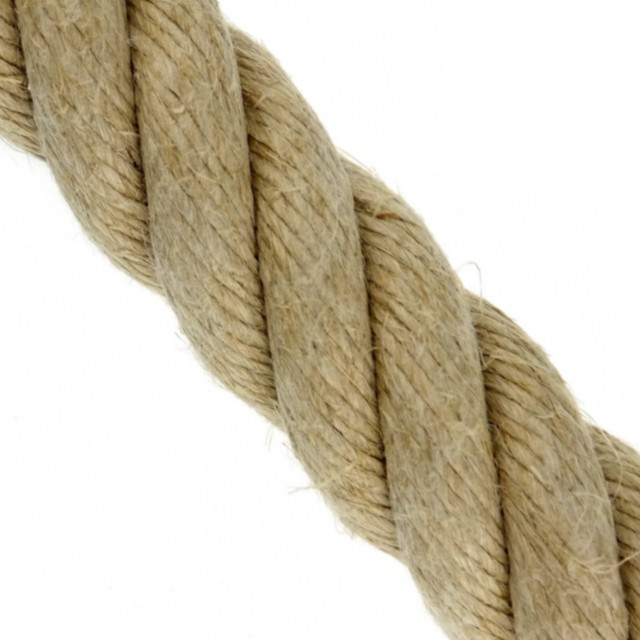
\includegraphics[width=0.2\textwidth]{Picture/hanfseil.png} & 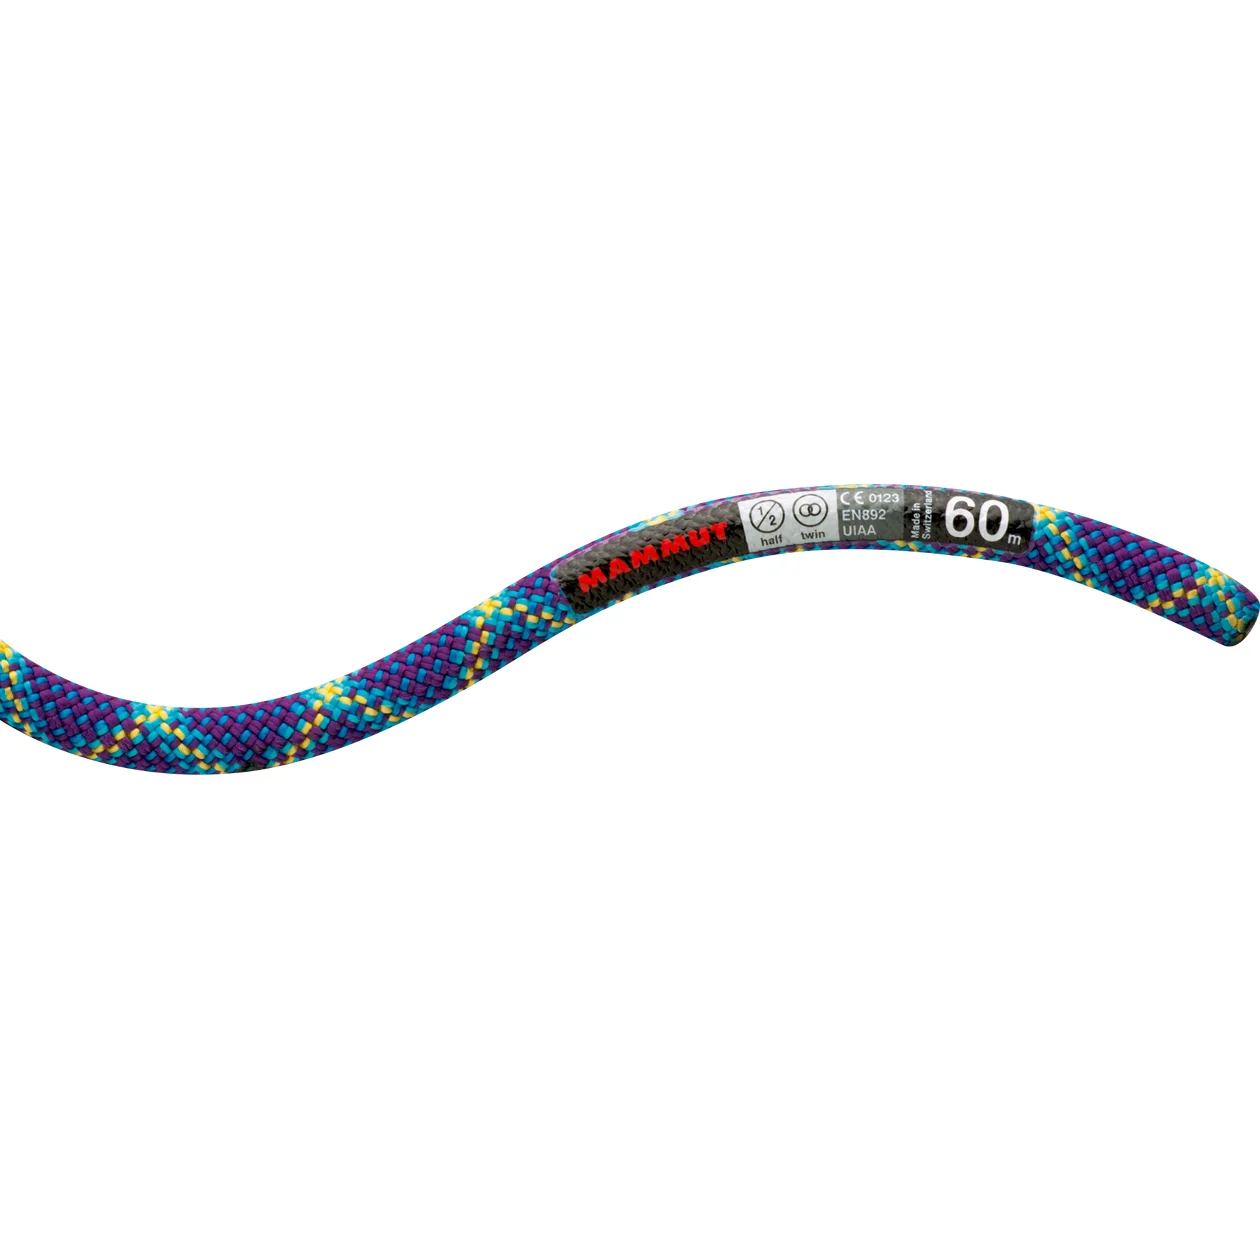
\includegraphics[width=0.2\textwidth]{Picture/bergseil.png} & 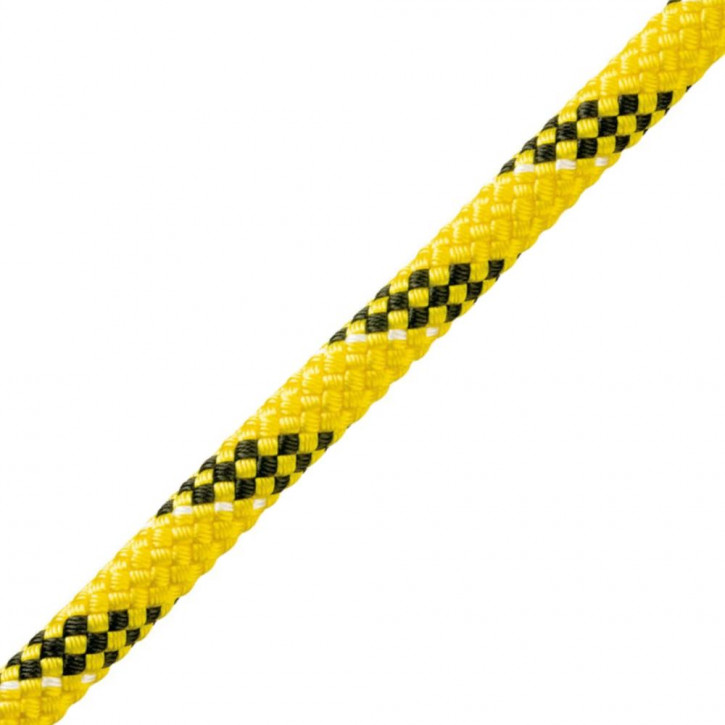
\includegraphics[width=0.2\textwidth]{Picture/statikseil.png} \\\hline
     Merkmal & braun, gedreht & farbig, geflochten & farbig, geflochten \\\hline
     Anwendung & Pioniertechnik, Seilbrücken & Abseilen & Seilbahnen, Strickleiter \\\hline
     Dehnung & gering & gross & gering \\\hline
     Temperatur- beständigkeit & $\approx$ 200$^\circ$C & $\approx$ 100$^\circ$C & $\approx$ 100$^\circ$C \\\hline
     Reissfestigkeit (trocken 10mm) & 800 kg & 2000 kg & 3000 kg \\\hline
     Material & Naturfaser & Kunstfaser (Nylon, Polyamid) & Kunstfaser (Nylon) \\\hline
     Scheuerfestigkeit & gut & empfindlich & gut \\\hline
     Verrotungs- beständigkeit & schlecht & gut & gut \\\hline
     Wasseraufnahme & viel (verkürzt sich) & wenig & wenig \\
\end{tabularx}
\end{center}
Die Seilpflege ist ein weiterer sehr wichtiger Aspekt wenn es um Seile geht, damit diese noch lange halten und auch sicher für den Gebrauch sind. Die fünf wichtigsten Sachen hierbei sind:

\begin{enumerate}
    \item Stehe nicht auf Seile
    \item Reinige Seile regelmässig (trocken)
    \item Schütze Seile vor Schmutz, Feuchtigkeit und direkter Sonnenbestrahlung
    \item Lagere Seile trocken und vor Sonnenlicht geschützt
    \item Lasse Seile nie über scharfe Kanten laufen
\end{enumerate}

\subsubsection{Knoten}

Genau wie bei den Seilen gibt es auch bei den Knoten einige Sachen auf die man achten sollte wenn man einen macht:
\begin{itemize}
    \item Befestige alle Knoten
    \item Ein Knoten halbiert die Tragfähigkeit eines Seiles
    \item Lasse am Knotenende genügend freies Seil
    \item Bringe einen Stecken beim Knoten in zwischen die Verbindung um den Knoten nach der Belastung wieder öffnen zu können.
\end{itemize}

Nun aber zu einer Tabelle mit den wichtigsten Knoten und ihren Eigenschaften:
\begin{center}
\begin{tabularx}{\textwidth}{X|X|X|X}
    \textbf{Name} & \textbf{Verwendung} & \textbf{Positive Eigenschafte} & \textbf{Negative Eigenschaften} \\\hline
    Samariter & Verbindung gleich dicker Seile & Einfach, Flach, leicht straffzuziehen & Öffnet sich bei grosser Belastung \\\hline
    Weber & Verbindung ungleich dicker Seile & Einfach zu knöpfen, leicht straffzuziehen & Öffnet sich bei grosser Belastung\\\hline
    Fischer/ Spierenstich & Verschiebbare Verbindung zweier ungleich dicker Seile & Hält sicher, kleine verringerung der Reissfestigkeit & Schwer zu öffnen \\\hline
    Gesteckter \footnote{Kann um einen Baum geknöpft werden} Achter & Schlinge zum Anseilen & Hält sicher, gut zum Öffnen & - \\\hline
    Bretzeli & Seilbefestigung an dünnen Gegenständen & Schnell geknöpft & Mühsam zu öffnen \\\hline
    Maurer & Seilbefestigung an dicken Gegenständen & Einfach zu öffnen & Nur eine Zugrichtung, Hält nur bei Belastung \\\hline
    Fläschli/Päckli & Zulaufende Schlinge für Pakete, Spanner, Strickleitern & Einfach zu knöpfen & Nur eine Schlaufen und Zugrichtung, mühsam zum öffnen \\\hline
    Fuhrmann & Zulaufende Schlinge für Spanner & Besser lösbar als Flächli/Päckli & Nur eine Schlaufen und Zugrichtung, mühsam zum öffnen \\\hline
    Anker & Befestigung einer Schlaufe & Einfach zu knöpfen & Seitliches verrutschen, gleicher Zug an beiden Enden \\\hline
    Halbmastwurf & Abseilen von Lasten & Gute Kontrolle von Lasten & Schnell falsch geknöpft, schwere Handhabung \\\hline
    Achterschlinge/ Mastwurf & Fixieren eines Seiles & Hält sehr gut, schräger Zug möglich & Mühsam zu öffnen \\\hline
    Schachbrett-/Freundschafts- knoten & Zierknoten zum Binden der Pfadikrawatte & Flacher Knoten & Mühsam zu öffnen \\
\end{tabularx}
\end{center}

\subsubsection{Blachen und Zelte}
Bei den Pfadfindern werden häufig Zelte mit Blachen und Zelteinheiten gebaut. Mit Zelteinheiten sind Säcke mit 3 Zeltstangen und 3 Heringen gemeint. Mit Blachen hingegen sind Militärblachen gemeint welche einen Fläche von circa 1.63 m $\cdot$1,65 m haben. Blachen sind circa 1.25kg schwer (nass bis zu 2.5kg) und haben 32 Löcher und 64 Knöpfe. Auch hier ist die Pflege sehr wichtig, so sollte man schmutzige Blachen zuerst trocknen lassen und danach abbürsten. Ausserdem sollte man nicht auf Blachen treten und sie nicht waschen, da beides die Imprägnierung kaputt macht. \par Dies ist eine Tabelle mit den häufigsten anwendungen von Blachen:

\begin{center}
\begin{tabularx}{\textwidth}{X|X|X|X}
    \textbf{Name} & \textbf{Anwendung} & \textbf{Material} & \textbf{Hinweise} \\\hline
    Blachenbund & Lagerung von 10 Blachen & 10 Blachen & - \\\hline
    Sarg & Gepäckunterstand, Windschutz für 1 Person & 1 Blache, 2 Zelteinheiten, Schnur & Sehr klein \\\hline
    Gotthardschlauch & Schlafstelle für 3 Personen, Materialunterstand & 3 Blachen, 2 Zelteinheiten, Schnur & Ist beliebig erweiterbar \\\hline
    Firstzelt & Gepäckunterstand & 2 Blachen, 2 Zelteinheiten, Schnur & Ist beliebig erweiterbar \\\hline
    Berliner & Schlafstelle für 5 Personen & 8 Blachen, 4 Zelteinheiten, Schnur & Wärmstes Blachenzelt \\\hline
    Sarasani & Aufenthaltszelt, Kochzelt & 27 Blachen, 1 Mittelpfosten, Schnur, 2 Seile, 15 Armierungseisen & Kann beliebig vergrössert werden \\ 
\end{tabularx}
\end{center}

\subsection*{Karte und Kompass}
\subsubsection{Grundsatz}
Die Schweiz hat ein eigenes Koordinaten System welches nach der Sternwarte Bern (2 600 000 /1 200 000) ausgerichtet ist. Das Schweizer Koordinatensystem ist zudem rechteckig was bedeutet, dass jeder Punkt der Schweiz mit einer x und einer y Koordinate angegeben werden kann. Bei den Karten der Schweiz ist Norden immer oben und sie sind in acht Massstäbe unterteilt, 1:10 000, 1:25 000, 1:50 000, 1:100 000, 1:200 000, 1:300 000, 1:500 000 und 1:1 000 000. Der Massstab ist hierbei $\frac{Kartenstrecke}{Naturstrecke}$, für die Pfadfinder sind allerdings praktisch nur die 1:25 000 und 1:50 000 wichtig da sie nicht so grosse strecken zurücklegen. Auf Karten werden ausserdem Höhenkurven verwendet welche es dem Benutzer ermöglichen anhand einer Karte abzuschätzen wie steil ein Gelände ist, zwischen zwei Höhenkurven liegt immer eine bestimmte Äquidistanz welche zwischen 10m und 50m variiert. 

\subsubsection{Koordinaten bestimmen}
Zum bestimmen der Koordinaten eines Punktes auf der Karte verwendet man ein Hilfsmittel namens Kartenmassstab, dieser ermöglicht es einem direkt strecken auf einer Karte einzuzeichnen. Um die Koordinaten zu bestimmen sucht man nun zuerst die Grobkoordinaten des Feldes in welchem der Punkt ist den man sucht. Danach liest man mit dem Kartenmassstab die genauen Koordinaten der x und y Achse ab. \par Um einen Punkt mithilfe von Koordinaten zu finden sucht man zuerst das richtige Feld in dem der Punkt liegen wird und bestimmt danach den Ort eines Punktes in dem man die genauen x und y Werte mithilfe des Kartenmassstabs in die Karte einträgt.

\subsubsection{Signaturen}

Signaturen auf einer Karte sind Symbole welche für ein Objekt in der Realen Welt steht. So steht zum Beispiel ein einfaches Quadrat auf einer Karte für ein Haus. Diese Signaturen sind dafür verantwortlich, dass man sich in einer unbekannten Umgebung nur mit einer Karte zurechtfindet. Auf den Karten gibt es auch immer auf der Rückseite ein Verzeichnis der wichtigsten Signaturen und sonst kann es auch online gefunden werden\cite{oa_zeichenerklarung_nodate}.

\subsection*{Samariter}
Beim Samariter geht es darum erste Hilfe leisten zu können. Deshalb ist das Vorgehen auch sehr wichtig, um das einfach Verständlich zu machen gibt es das Ampelsystem. Zuerst ist die Ampel Rot, das bedeutet schauen, spricht das Ausmass des Unfalls betrachten und mögliche Gefahren für sich selbst. Danach ist die Ampel Orange was bedeutet denken, hier geht es darum einen Plan zu machen um ihn danach umzusetzen. Am Ende kommt noch Grün wo es dann heisst das umsetzen was bei Orange geplant wurde. \par
Beim Handeln ist das Alarmieren sehr wichtig, denn wenn man Falsch oder gar nicht allarmiert kann dies im schlimmsten Fall Leben kosten. Deshalb lernen Pfadfinder auch die wichtigsten Notrufnummern. Diese wären 112 für den Europäischen Notruf, 117 für die Polizei, 118 für die Feuerwehr, 144 für die Ambulanz, 1414 für die REGA und 145 für das Tox-Zentrum. Wenn man allerdings die richtige Nummer gewählt hat ist das ganze Alarmieren noch nicht fertig und man muss noch die wichtigsten Fragen beantworten welche die 6 W-Fragen sind: Wer?, Was?, Wo?, Wann?, Wieviele? und Weiteres?. \par
Nach dem Alarmieren kümmert man sich um den Patient, hierbei gibt es die Regel ABC. A steht für Atemwege, hier wird geschaut ob der Patient in der Lage ist zu Atmen. B steht für Beatmen, dies wird durchgeführt wenn der Patient nicht mehr Atmet. C steht für CPR was eine Herzmassage ist, diese wird durchgeführt wenn das Beatmen nicht funktioniert hat. \par
Fals die Atmung funktioniert und ein Patient starke Blutungen oder Schmerzen hat muss man teilweise einen Verband machen. Hierbei gibt es drei Arten, einen Druckverband, einen Stützverband oder einen Deckverband. Der Druckverband übt starken Druck auf die Wunde aus und kann so starke Blutungen stoppen. Der Stützverband dient als Stütze für ein verletztes Körperteil. Der Deckverband dient als schutz vor Verunreinigungen der Wunden.

\subsection*{Übermittlung}
Die Übermittlung befasst sich hauptsächlich mit dem Morsecode, beim Morsecode werden Buchstaben in Punkt und Strich umgewandelt und so versendet. Der grosse Vorteil von Morsen ist, dass man es auf sehr viele Verschiedene arten machen kann, so kann man zum Beispiel Morsetafeln verwenden oder auch Taschenlampen im Dunkeln. Zur Umwandlung von Buchstaben zu Morsecode wird ein Morseschlüssel verwendet.
\begin{figure}
    \centering
    \includegraphics[width=0.5\linewidth]{Picture/morseschlüssel.png}
    \caption{Morseschlüssel}
\end{figure}
\par
Ein weiterer Aspekt der Übermittlung sind die Geheimschriften welche im Thilo \cite{noauthor_thilo_2014} sind. Eine dieser Verschlüsselungen ist die Cäsarverschlüsselung bei der alle Buchstaben um eine bestimmte Anzahl Buchstaben im Alphabet verschoben werden. Eine andere Verschlüsselung nennt sich Quadratgittern, hierbei schreibt man die Nachricht waagrecht in ein Raster und sendet sie danach Senkrecht gelesen. Die letzte Verschlüsselung nennt sich Koordinatengitter, hierbei wird das Alphabet in ein Koordinatengitter geschrieben, danach bekommt jede Zeile und Spalte einen Buchstaben als Koordinate. Die Nachricht ist danach die Koordinaten aller Buchstaben der Nachricht zusammen gehängt.

\subsection*{Pfadigeschichte}
\subsubsection{Geschichte der Pfadibewegung}
Robert Stephenson Smyth Baden-Powell, der Gründer der Pfadfinder, wurde am 22. Februar 1857 in London geboren. Er viel durch die Aufnahmeprüfungen der Universität und entschied sich Kariere im Militär zu machen. Er wurde in der Kolonie Indien stationier wo er auf Spione oder Scouts aufmerksam wurde und deren wichtige Funktion im Kampfgeschehen erkannte. Später wurde er nach Südafrika verlegt wo er zum ersten mal seine eigenen Scouts ausbilden konnte, aber immer noch im militärischen Umfeld. Als Baden-Powell, nun besser bekannt als BiPi, eine Stadt aus der Belagerung befreien musste setzte er seine Scouts erstmals im Gefecht ein und er war erstaunt wie gut sie ihre Aufgaben bewältigten. \par Zurück in England beendete BiPi seine Militärische Kariere und sagte: \glqq Am Ende meiner Kariere begann ich, die Kunst, junge Leute zu lehren, wie man Krieg macht, umzuwandeln in die Kunst junge Leute zu lehren, in Frieden zu leben; Pfadi ist weit entfernt vom Krieg\grqq \par
Im Jahre 1907 organisierte er das erste Pfadilager für Jungen auf der Insel Brownsea. Nach dem riesigen Erfolg dieses Lager schrieb er das Buch Pfadfinder. Das Buch war ein solcher Erfolg, dass überall in England neue Pfadigruppen entstanden und 1909 auch die Mädchen dazu kamen unter dem Namen Guides. \par Im Jahre 1912 heiratete BiPi Olave Saint Clair Soames welche als Chief Guide die Leitung über die Pfadfinderinnen übernahm. 1920 fand das erste Jamboree \footnote{Pfadilager mit Abteilungen von der ganzen Welt} statt, es nahmen Jugendliche aus 34 Ländern teil. Später wurde BiPi zum World Chief ernannt. Die Pfadibewegung explodierte danach und um 1993 gab es etwa 25 Millionen Pfadi in über 150 Ländern. 

\subsection{Java}
Die Programmiersprache in der diese Projekt geschrieben wird ist Java. Java existiert seit 1995 und in dieser Sprache sind sehr viele Apps programmiert worden\cite{noauthor_what_nodate}. Java ist so aufgebaut, dass wenn man ein Programm darin laufen lässt, eine Virtuelle Maschine gestartet wird. Dies hat zur Folge, dass nicht der Computer der das Programm ausführt abstürzt bei einem Fehler sondern die Virtuelle Maschine\cite{wikipedia-autoren_java_2024}. Auch ist Java eine Programmiersprache die für die \gls{oop} entwickelt wurde. 

\subsubsection{Wichtige Syntax}
In Java gibt es einige wichtige Grundbegriffe die man verstehen muss um die Programme zu verstehen was sie machen. Etwas sehr wichtiges ist, dass immer am Ende einer Zeile mit einer Anweisung ein Semikolon kommt und dass der Code innerhalb von Funktionen immer in geschweiften Klammern geschrieben ist. Auch sehr wichtig ist, dass man immer eine Klasse und eine Main Methode hat in der man das Programm schreibt. Um in einem Programm etwas auszugeben schreibt man System.out.println("Text");\cite{programmieren_lernen_java_2021}.
\begin{minted}{java}
//Die Main Klasse ist die Hauptklasse des Programms
public class Main {
    //Die Main Methode ist der Einstiegspunkt in das Programm
    public static void main(String[] args) {
        System.out.println("Hello World!");
        //Diese Programm liefert den Output: Hello World!
    }
}
\end{minted}

\subsubsection{Datentypen}
Die Datentypen in Java sind in 2 Kategorien aufgeteilt, primitive Datentypen und Referenzen Datentypen. Primitive Datentypen gibt es acht Byte, Short, Integer, Long, Float, Double, Character und Boolean. Die ersten vier Datentypen sind dabei für die ganzzahligen Zahlen verantwortlich, hierbei kann in einem Byte eine Zahl im Bereich von $-2^7$ bis $2^7-1$ gespeichert werden, in einem Short eine Zahl im Bereich von $-2^{15}$ bis $2^{15}-1$, in einem Integer eine Zahl im Bereich von $-2^{31}$ bis $2^{31}-1$ und in einem Long eine Zahl im Bereich von $-2^{63}$ bis $2^{63}-1$. Somit ist es also nur eine Frage des Speicherplatzes und der grösse der Zahl welchen dieser Datentypen man nimmt, als Standard wird meist der Integer als Mittelwert verwendet. In diesen Datentypen können aber keine Kommazahlen gespeichert werden, diese werden nämlich in einem Float oder in einem Double gespeichert. Auch diese beiden Datentypen unterscheiden sich nur in dem Bereich an Zahlen die sie Speichern können, ein Float deckt den Bereich von $\pm 1.4 \cdot 10^{-45} \text{bis} \pm 3.4 \cdot 10^{38}$ ab und ein Long den Bereich von $\pm 4.9 \cdot 10^{-324} \text{bis} \pm 1.7 \cdot 10^{308}$. Hierbei hat sich als Standard der Double durchgesetzt.\par 
Die zwei verbleibenden Datentypen sind der Character und der Boolean. Der Character kann hierbei Zeichen in sich Speichern, hierbei ist es allerdings nicht nur möglich Buchstaben des lateinischen Alphabets zu verwenden, es gehen auch Zahlen, Spezialzeichen wie @ oder Unicode wie $\backslash$03A9 für $\Omega$. Der letzte primitive Datentyp ist der Boolean, der Boolean hat nur zwei Status True und False oder in Computersprache 1 und 0\cite{studyflix_java_nodate}.\par
Der zweite Typ von Datentypen sind die Referenzen Datentypen, zu ihnen gehören alle anderen Datentypen wie zum Beispiel Klassen und ihre Objekte, Interfaces, Arrays, Strings, etc. All diese Datentypen setzen sich aus mehreren Primitiven Datentypen zusammen, so sind Strings zum Beispiel einfach viele Character aneinander gehängt.

\subsubsection{Variablen}
In Java gibt es wie in den meisten Programmiersprachen Variablen. Variablen sind dafür da Werte in sich zu Speichern. Der Wert einer Variable kann überschrieben werden, der Datentyp des Wertes muss aber gleich bleiben. Variablen müssen immer Deklariert und Definiert werden damit man sie benutzen kann, dies kann in zwei unterschiedlichen Zeilen geschehen oder in einer.
\begin{minted}{java}
public class Main {
    public static void main(String[] args) {
        int integerValue;
        //Deklarierung der Variable intergerValue
        //Zuerst wir der Datentyp definiert, dann der Variablenname
        integerValue = 1;
        //Definition der Variable intergerValue
        //Der Variablenname ist gleich dem Variablenwert
        double doubleValue = 1.0;
        //Deklaration und Definition der Variable doubleValue in einem Schritt
        //Zuerst wird der Datentyp genannt, dann der Variablenname ist gleich 
        //dem Variablenwert
    }
}
\end{minted}
Variablen können ausserdem miteinander zusammengerechnet oder zusammengeführt werden\cite{programmieren_lernen_java_2021}.
\begin{minted}{java}
public class Main {
    public static void main(String[] args) {
        int intValue = 1;
        //Hier wird eine Variable mit dem Namen intValue und dem Wert 1 erstellt
        int intValue2 = 2;
        //Hier wird eine Variable mit dem Namen intValue2 und dem Wert 2 erstellt
        int intValue3 = intValue + intValue2;
        //Hier wird eine Variable mit dem Namen intValue3 und dem Wert von 
        //intValue + intValue2 erstellt
    }
}
\end{minted}

\subsubsection{Verzweigungen}
Verzweigungen in Programmiersprachen sind dafür da um Fälle zu lösen in denen es verschiedene mögliche Szenarien gibt bei denen man unterschiedliche Sachen machen muss. Hierfür gibt es zwei Methoden die meistens verwendet werden, die eine ist das If Else Anweisung und die andere ist  nennt sich Switch case. Die If Else Anweisung ist dafür da um zwei Werte zu vergleichen, wenn der Vergleich ergibt, dass sie identisch sind wird der If Teil der Funktion durchgeführt und wenn sie nicht identisch sind wird der Else Teil durchgeführt. Es kann allerdings noch einen dritten Teil geben, einen Else-If Teil, dieser ist dafür da einen zweiten Vergleich zu machen um zu schauen ob dieser stimmt.
\begin{minted}{java}
public class Main{
    public static void main(String[] args) {
        if (2 == 1){
            //Wenn 2 gleich 1 ist, dann wird das ausgeführt
        } else if (2 == 2) {
            //Wenn 2 gleich 2 ist, dann wird das ausgeführt
        } else {
            //Wenn nichts davon zutrifft, dann wird das ausgeführt
        }
    }
}
\end{minted}
Die Andere häufig Verwendete Methode des Switch cases macht im Grundsatz genau das Selbe. Hier wird eine Variable in den Switch teil herein gegeben und dann wird für verschiedene Zustände dieser Variable verschiedene Zeilen Code ausgeführt\cite{programmieren_lernen_java_2021}.
\begin{minted}{java}
public class Main{
    public static void main(String[] args) {
        int var;
        switch (var) {
            case 1:
                //Wenn die Variable var den Wert 1 hat, wird dieser Code 
                //ausgeführt
                break;
            case 2:
                //Wenn die Variable var den Wert 2 hat, wird dieser Code 
                //ausgeführt
                break;
            default:
                //Wenn die Variable var keinen der Werte 1 oder 2 hat, 
                //wird dieser Code ausgeführt
        }
    }
}
\end{minted}

\subsubsection{Schleifen}
Schleifen in der Programmierung sind dafür da gewisse Zeilen eines Programms mehrfach zu wiederholen. Genau wie bei den Verzweigungen gibt es auch hier zwei typen von schleifen die sich durchgesetzt haben die While und die For Schleife. Die While Schleife macht einen Teil des Programms so lange bis eine Funktion nicht mehr erfüllt ist. Die For schleife wiederholt einen Teil des Programms so lange bis er durch alle Glieder einer bestimmten Reihe oder eines Arrays durch ist oder bis die Variable die man der Schleife gibt einen bestimmten Wert übersteigt\cite{freecodecamporg_android_2020}.
\begin{minted}{java}
public class Main{
    public static void main(String[] args) {
        
        int count = 0;
        while (count < 10) {
            //Solange die Bedingung count ist kleiner als 10 erfüllt ist, wird
            //der Code wiederholt
            //Hier ist der Code der wiederholt werden soll
            count++;
            //Count wird um 1 erhöht und es wird wieder geprüft, ob die 
            //Bedingung erfüllt ist
        }
        
        for (int i = 0; i < 10; i++) {
            //Solange die Bedingung i kleiner als 10 erfüllt ist, wird der 
            //Code wiederholt, i wird um 1 erhöht
            //Hier ist der Code der wiederholt werden soll
        }
\end{minted}
\newpage
\begin{minted}{java}
        String word = "Hallo";
        for (char c : word.toCharArray()) {
            //Solange es noch Zeichen im Wort gibt, wird der Code wiederholt
            //Hier ist der Code der wiederholt werden soll
        }
    }
}
\end{minted}

\subsubsection{Klassen und Objekte}
Java ist eine Sprache die auf die \gls{oop} ausgelgt wurde. Bei der \gls{oop} geht es darum eine Klasse zu definieren und dann mit den Objekten dieser Klasse weiter zu Programmieren. Innerhalb einer Klasse gibt es sogenannte Methoden, dies Methoden sind Teile eines Programms die ein Objekt dieser Klasse ausführen kann. So könnte man zum Beispiel eine Figuren klasse erstellen mit der Methode jump welche ausgibt dass der Spieler springt. Dadurch da wir das ganze aber als Klasse gemacht haben können wir nun nicht nur ein Objekt dieser Figuren Klasse haben sondern wir können mehrere Figuren haben die alle über die Methode jump verfügen.
\begin{minted}{java}
//Datei: Main.java
public class Main{
    public static void main(String[] args) {
        //Ein neues Objekt der Klasse Figuren wird erstellt mit dem Namen Mario
        Figuren Mario = new Figuren("Mario");
        //Die Methode jump() wird aufgerufen über das Objekt Mario
        Mario.jump();

        //Ein neues Objekt der Klasse Figuren wird erstellt mit dem Namen Luigi
        Figuren Luigi = new Figuren("Luigi");
        //Die Methode jump() wird aufgerufen über das Objekt Luigi
        Luigi.jump();
    }
}

//Datei: Figuren.java
public class Figuren {
    private String name;

    public Figuren(String name){
        this.name = name;
    }

    public void jump(){
        System.out.println(name + " springt");
    }
}

//Output:
//Mario springt
//Luigi springt
\end{minted}

\subsection{Android Studio}
Android Studio ist eine Desktop App für die Entwicklung von Android Apps. In Android Studio kann entweder in Java oder in Kotlin Programmiert werden. Android Studio ist eine JetBrains IDE \footnote{Integriertes Entwicklungs Umfeld} was bedeutet, dass es man eine direkte Verbindung mit GitHub aufbauen kann um so das Projekt immer auf GitHub auf dem neusten Stand zu haben\cite{freecodecamporg_android_2020}.

\subsubsection{Struktur}
Innerhalb von Android Studio gibt es drei Arten von Dateien welche miteinander verbunden sind, zum einen gibt es die Ressource Dateien, zum andern gibt es die Layout Dateien und sonst gibt es noch die Java Dateien. Die Ressource Dateien sind Dateien wie Bilddateien oder Themendateien die die Grundlage der Informationen Bilden auf der die ganze App basiert. Die Layout Dateien sind dafür da, dass es Objekte auf dem Bildschirm des Users gibt. So steht zum Beispiel in einer Layout Datei, wo ein Button ist, was er für einen Hintergrund hat, wie er heisst und wie gross er ist. In den Java Dateien werden dann den Objekten aus den Layout Dateien Funktionen gegeben. So wird hier das Programm geschrieben das ausgeführt wird wenn man eine Button drückt\cite{freecodecamporg_android_2020}.

\subsubsection{Layouts}
Bei den Layouts in Android Studio gibt es auch noch Unterschiede. So gibt es drei Hauptarten von Layouts, das Constraint Layout, das Relative Layout und das Linear Layout. Bei dem Constraint Layout werden die Objekte immer mit Verbindungen zu anderen Objekten Positioniert. Beim Relative Layout werden die Objekte immer relativ zu den anderen positioniert, so wird hier häufig mit Abständen zu anderen Objekten geschafft. Das letzte Layout ist das Linear Layout, beim Linear Layout werden die Objekte immer in einer Fixen Reihe Positioniert und es kann nur der Abstand zum vorherigen Objekt verändert werden. Bei all diesen Layouts müssen allerdings die Attribute der Objekte gleich angegeben werden\cite{freecodecamporg_android_2020}.